% This work is licensed under
% http://creativecommon.org/licenses/by/3.0/
\section{The geomorphic view of networking}
\label{sec:sec2}

The geomorphic
view of networking was originally inspired by the work of Day \cite{pna},
although we have made many changes and additions in both content and
presentation.
In this common framework for describing networks,
the module is a
{\it layer}, and a network architecture is a hierarchy of layers.

\subsection{Comparison with the Internet and OSI models}
Layers may seem familiar and obvious because both the classic Internet
architecture \cite{philo} and the
OSI reference model \cite{OSI}
also describe network architecture as a hierarchy of layers.
However,
our concept of a layer is very different.
As a preview of this section, our layer hierarchies differ from these
earlier ones in at least four ways:
\begin{itemize}
\item
The classic Internet architecture and the OSI reference model both have
a fixed number of levels.
In a geomorphic layer hierarchy, there can be any number of levels.
\item
In the earlier models, there is only one layer on each level, so there
is no distinction between layer and level.
In a geomorphic hierarchy, there can be multiple layers on the same
level.
\item
In the earlier models, each layer has a specific function that is
distinct from the functions of other layers.
In the geomorphic view
each layer is a microcosm of networking, containing all of the basic
components and functions in some form.
In different layer instances there are different versions of these
basic ingredients, used at
different levels, with different scopes, and for
different purposes.
\item
Most people interpret the earlier models as describing the data
plane of networking only.
The control plane is seen as separate and not modularized in the
same way.
In the geomorphic view, each layer---being a microcosm of
networking---has a data plane and a control plane.
Layers decompose both planes into modules.
\end{itemize}
Figure~\ref{fig:geoname} illustrates these differences, and also
shows how the ``geomorphic'' view got its name.
The complex arrangement of layers, with overlapping, abutting, and
bulging shapes, can resemble the complex arrangement of layers in the
earth's crust.

\begin{figure}
\centering
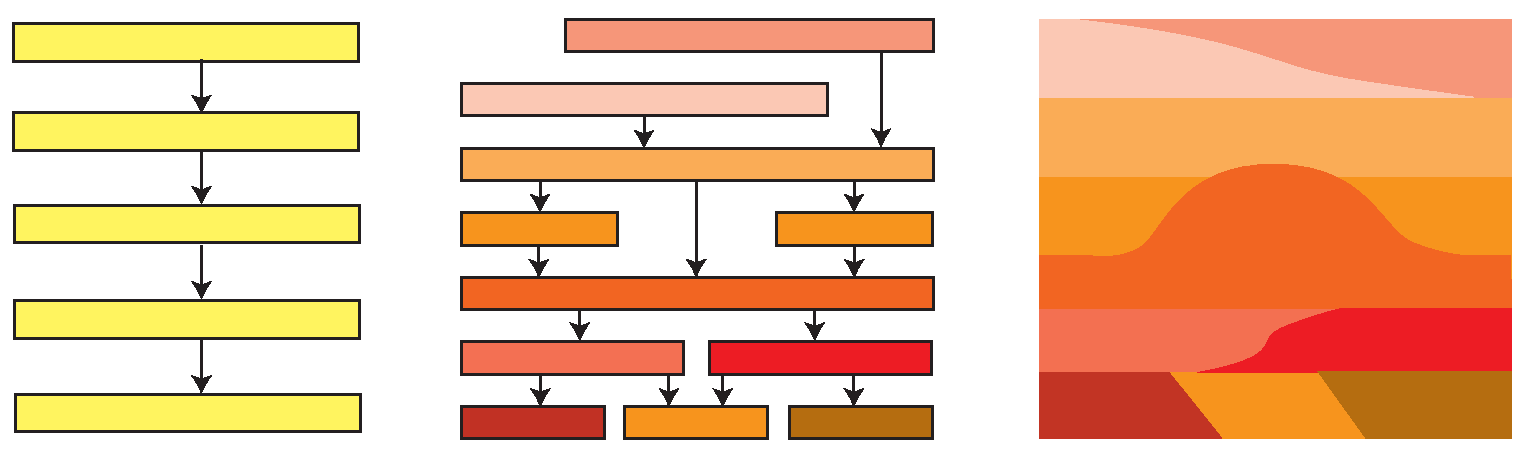
\includegraphics[scale=0.45]{figures/geoname.pdf}
\caption{Arrangement of layers in the classic Internet architecture
(left), the geomorphic view (middle), and the earth's crust (right).}
\label{fig:geoname}
\end{figure}

\subsection{Components of a layer}
\label{sec:layercomponents}

A layer has {\it members}, each of which has a unique and persistent
{\it name} within the layer.
For example, Figure~\ref{fig:layer} is a snapshot of a layer with five
members, each having a capital letter as a name.
In general a member is a concurrent process, {\it i.e.,} a locus
of state and control with the potential for autonomous action.

The members of a layer communicate with each other through {\it links},
shown by lines in Figure~\ref{fig:layer}.
A link is a communication channel.

\begin{figure}
\centering
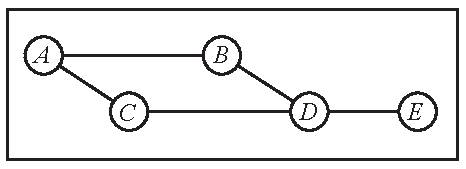
\includegraphics[scale=0.80]{figures/littlelayer.pdf}
\caption{Members and links of a layer.}
\label{fig:layer}
\end{figure}

One of the two primary functions of a layer is to enable members to send
messages to each other.
This function is accomplished by a {\it forwarding protocol},
which runs in all members and has operations for sending and
receiving messages over the links.

In general, a layer does not have a link between each pair of members.
Such a layer needs {\it routes}
indicating how one member can reach another through links and
intermediate members.
For example, ({\it A, B, D, E} ) is a route from {\it A} to {\it E}.
If {\it B} receives a message that is destined
for {\it E}, its forwarding protocol uses the route information
to forward the message to {\it D} on its way to {\it E}.

The {\it routes} are shared state of the layer, and a simple 
geomorphic description need say no more about them. 
To provide more realistic detail, in a real layer the {\it routes}
information is often distributed over forwarding tables found in
the individual members.

The other primary function of a layer is to implement enriched
end-to-end
communication services on top of its bare message transmission.
This function is carried out by a {\it session protocol}.
The forwarding protocol can be unreliable, especially if links are
dynamic and the current routes are obsolete.
A session protocol can provide services including reliability,
FIFO delivery,
and quality-of-service guarantees.
Figure~\ref{fig:impl} shows a session between endpoints {\it a}
and {\it e} of the lower layer.

A {\it channel} is an instance of a communication
service.
Both links and sessions are channels.
A layer can implement its own links internally, and a
layer can implement its sessions for the benefit of its own
members.

Most commonly, however, a link in one layer is
implemented by a session in another layer,
as shown in Figure~\ref{fig:impl}, placing the other
layer lower in the {\it ``uses'' hierarchy}.
If an underlay (lower layer) is implementing a link for an overlay
(higher layer), then the basic attributes of the channel must be
stored in the states of both layers.
In the overlay, the channel object is one of its {\it links}.
In the underlay, the channel object is one of its {\it sessions}.
There must be two names for the sets of channels of interest to a layer,
because a typical layer both uses {\it links} and 
implements {\it sessions}.

For a link in an overlay to be implemented by a session in an underlay,
both endpoint {\it machines} must have members in both layers,
as shown in Figure~\ref{fig:impl}.
The boundary of a
{\it machine} is the boundary of an operating system that provides fast,
reliable communication between members of different layers on the machine.
This fast, reliable operating-system
communication is the foundation on which networked
communication is built.\footnote{Although layer members have been
described as concurrent processes, they are not usually ``processes''
as defined by the operating system; processes in an operating system
have many more properties and associations than layer members do.  
A virtual machine can be regarded as a {\it machine}, in which case
communication through the hypervisor and soft switch of the physical
machine is regarded as networked communication.}

\begin{figure}
\centering
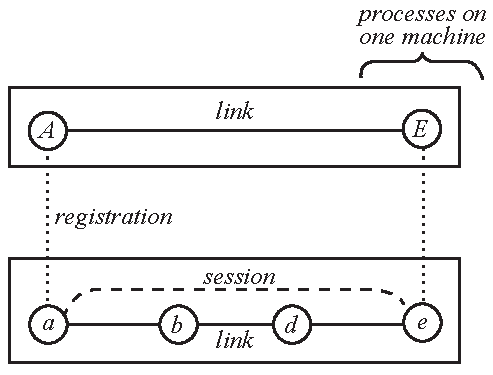
\includegraphics[scale=0.80]{figures/impl.pdf}
\caption{Implementation of a link in an overlay by a session in an
underlay.}
\label{fig:impl}
\end{figure}

The relation between an overlay member and an underlay member on the
same machine is called {\it registration}.
Registrations must be stored in the state of both layers.
In the overlay a registration is recorded as an {\it attachment}, 
which says that the overlay member is attached to the network through
a particular lower layer.
In the underlay a registration is recorded as a
{\it location}, 
which says that a particular member of a particular overlay is attached to
the network at a particular member (its location) of this layer.

The session protocol creates and maintains {\it sessions} data in its
layer, and uses {\it locations} data.
For example, in Figure~\ref{fig:impl}, {\it A} sent a request to {\it a}
for a session with {\it E}.
To create this session, {\it a} learned from its layer's {\it locations}
that {\it E} is currently located at {\it e}.
Messages sent from {\it A} to {\it E} through the link in the overlay
travel through {\it a, b, d,} and {\it e}; the first and last steps
uses operating-system communication, while the middle three steps use
networked communication.

All the major components of a layer are shown in
Figure~\ref{fig:table}.
The forwarding and session protocols perform the two primary functions
of the layer.
These protocols and their operations are collectively known as the
``data plane'' of the layer.
The network's data plane also includes the inter-layer interfaces
through which the endpoints of an implemented link transfer messages to 
and from the
implementing session.

There are six major state components, all of which 
can be dynamic.
We have seen that the session protocol creates and maintains
{\it sessions};
the other five are created and maintained by their own maintenance
algorithms.
The state and algorithms are collectively known as the ``control plane''
of the layer.
Note that the network's control plane also includes the inter-layer
interfaces through which the control algorithms communicate.

\begin{figure}
\centering
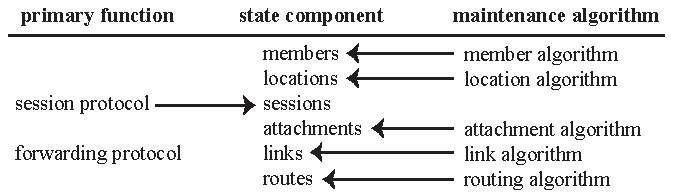
\includegraphics[scale=1.00]{figures/table.pdf}
\caption{Major components of a layer.  Arrows show which protocol
or algorithm writes a state component.}
\label{fig:table}
\end{figure}

\subsection{Layers within a network architecture}

Figure~\ref{fig:scope} shows a geomorphic view of the classic
Internet architecture.
The {\it scope} of a layer is its set of potential members.
For example, 
at the top level of the hierarchy, there are two application layers.
The scope of each layer is the set of potential processes running
software for that application.
These layers are pictured as overlapping because the horizontal
dimension is an approximation of geographical space, and both
applications can have members world-wide.
In particular, the registration lines in the diagram show that each
application has a member on one particular machine.

\begin{figure}
\centering
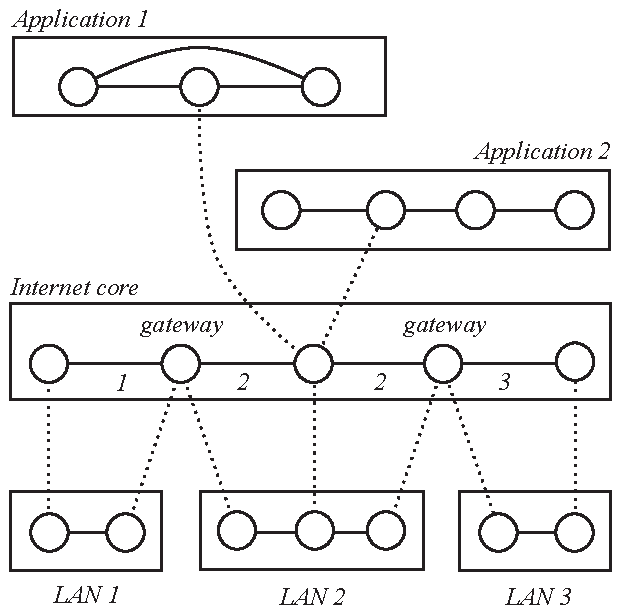
\includegraphics[scale=0.80]{figures/newip.pdf}
\caption{Geomorphic view of the classic Internet architecture.
Internet links are labeled with the LAN that implements them.}
\label{fig:scope}
\end{figure}

In the middle level of the hierarchy there is a single layer called
the ``Internet core.''
Its members are the IP interfaces of networked machines.
In this layer, IP (the ``network layer'' of the classic Internet
architecture) is the forwarding protocol, and TCP and UDP
(the ``transport layer'' of the classic Internet architecture)
are variants of the session protocol.

At the bottom level of the hierarchy there are local area networks
(LANs) with local scopes.
Each LAN member is an interface appropriate to the type of LAN.
For example, for an Ethernet LAN, the members are the Ethernet interfaces
of machines.
Figure~\ref{fig:scope} illustrates the point, made in the preview
of this section, that in the geomorphic view there can be multiple layers
at one level of the ``uses'' hierarchy.

Note that every member of the Internet core is attached to a member
of a layer at the bottom level.
Note especially that for two members of the Internet core layer to
be linked, both of those members must be attached to the same layer
at a lower level, so that the lower layer can implement the link.
This observation is important for understanding mobility.
A gateway in the Internet core layer is attached to multiple LANs, 
so it can forward messages from one LAN to another.

Because layers instantiated at different levels have different purposes,
they have different versions of the common components enumerated in
Figure~\ref{fig:table}.
For one
example, the best-known routing algorithms are found in the Internet
core, where their purpose is reachability.
Now consider a middleware layer, above the Internet core,
offering cloud services and other facilities for enterprise computing.
To provide security, this layer might have routing that ensures
that all messages
to a particular destination pass
through a particular filtering server.
Thus this layer has its own routing (control plane),
separate from Internet routing.
One of the major purposes of its routing is enterprise-specific
security.

This example
illustrates the points, made in the preview
of this section, that in the geomorphic view the number of levels
is not fixed (the middleware layer need not be present for the Internet
to work),
and that each layer can contain its own version of any basic
function or component of networking (such as routing).
In some layers, where a particular function or component is not
needed, its presence is vestigial.

For another example of a basic function with different forms in
different layers, low-level layers such as Ethernet
LANs provide
broadcast as a communication service.
In geomorphic terms, channels (links and sessions) can be multi-point
as well as point-to-point.
The main
services provided by the Internet core are point-to-point, while
an application layer might implement its own multi-party communication
service.\footnote{For simplicity, in the remainder of this chapter,
all communication channels are assumed to be point-to-point.
This is sufficient for a study of mobility.}

Today's Internet is host to many customized architectures running
simultaneously \cite{roscoe,spatscheck}.
Middleware is an important part of the ecosystem, while cloud services
and virtual private networks
add extra layers to the classic Internet architecture.
It is self-evident that fixed layer structures cannot describe
these architectures adequately.
The geomorphic view is intended not only to describe them,
but also to generate a design space including many others not yet
explored.

\subsection{Layers and mobility}
\label{sec:layers.and.mobility}

If asked to define network mobility, most people would say something
like, ``A mobile device continues to have network connectivity as it
moves geographically.''
For a simple Internet example, we can imagine a laptop that detaches
from one edge subnetwork, where it has one IP address, and re-attaches
to another edge subnetwork, where it has another IP address.

No layering is required to understand this scenario.
At the same time, technologically
the scenario is indistinguishable from a scenario
in which one laptop is tossed into a deep lake and another 
laptop is purchased new.

Clearly mobility is more than this.
As the mobile device detaches and re-attaches, we expect it to retain some
identity and credentials, so that it can be reached in some of the
same ways as
before, and has some of the same rights and capabilities as before.
The identity that is preserved is its membership in some layer, which
must not change.
What does change
is the attachment of this identifying
process to some process in some lower layer.

%JEN: references a figure in section 7.  intentional? move figure here?
The left column of Figure~\ref{fig:lift} (which appears later, in 
Section~\ref{sec:fig:lift}) shows the two forms that
this change of attachment can take.
In the top picture, a process {\it m} changes its registration from
one member of a lower layer to another member of the same layer.
The name {\it m} might be an application name, and {\it a1} and {\it a2}
might be IP addresses in an Internet core layer.
In the bottom picture, {\it m} changes its registration from
a member of one lower layer to a member of another lower layer.
Here {\it m} might be an IP address, and {\it a1} and {\it a2}
might be members of two different LANs.

This shows that layering is an intrinsic part of the study of
mobility, because it explains
what stays the same and what changes.
It will help us understand how a person can
call a friend's cellphone, even
though that friend has traveled hundreds of miles since the last call.

Even this is not sufficient to explain, however, how a person can talk
to a friend's cellphone {\it while the friend is traveling hundreds of
miles.}
To explain this aspect of mobility
it is necessary to focus on the communication channel
that is being preserved across mobility events.
As presented in Section~\ref{sec:layercomponents}, a communication
channel is most often used in one layer, where it is called a link,
and implemented in a lower layer, where it is called a session.
Here is another place where layering is intrinsic to the study of
mobility, explaining that the layer that benefits from mobility is
usually not the layer that has the responsibility of implementing it.

To summarize, there are two relationships on layer pairs that are
important in mobility.
There is a dynamic
registration relationship between an overlay with a mobile member
and the
underlays to which that member of the overlay is attached over time.
There is an implementation relationship between an overlay with a link
and the underlay whose session implements that link.
Two overlay/underlay pairs---in any given instance of mobility, they
must be the same overlay and underlay, right?

Wrong.  
Section~\ref{sec:sec3} will show that there are two patterns for mobility.
In one pattern the layer pairs coincide, and in the other 
they are different.
People are often confused by mobility because it is often over-simplified.
Mobility is easy to over-simplify when one is not explicit about the
layers involved.

\subsection{Mobility in the wild}

It might be said that the problem with mobility is not too few proposals,
but too many.
As mentioned in the introduction, the
total number is probably in the hundreds and growing.

In this chapter, the geomorphic view will provide a descriptive 
framework that imposes some order on this chaotic design space.
This works because every mobility proposal has a unique description
in terms of layers in the geomorphic view.

Unique description is achieved only because the geomorphic view is
precisely defined and precisely used.
For one example, in the geomorphic view there is one name space per
layer.
If any proposal has two different names for the same machine,
one higher-level and one lower-level, then those names must be in
the name spaces of two different layers.
For another example, in the geomorphic view there is no tunneling.
Tunneling is evidence that there are two distinct layers: a higher
layer in which the ``tunnel'' is a link, and a lower layer that
implements the link.

As a result, a geomorphic description of a network architecture might have
more layers than a different description, and some components of some
layers might be vestigial.
This is a cost, but in return we get many benefits, even beyond the
benefits of having a unique and comparable description of each proposal:
\begin{itemize}
\item
Each layer is simpler, with a minimum of {\it ad hoc} complications.
\item
Proposals that might seem very diverse fall into a few recognizable
patterns that apply at any level of the network stack.
\item
We can identify opportunities for re-use of formal models, 
formal analysis, and implementation code.
\item
Mobility is not the only networking challenge.
If other complex mechanisms are also described in terms of the geomorphic
view, we can make sure that they interact correctly.
\end{itemize}
Furthermore, redundancies in a description or model can be
removed by optimization in an implementation phase.
The trick is to understand and analyze the model first, then use the
analysis to determine which optimizations are safe.

This approach leads to differences from other literature on
mobility.
As exemplified by
\cite{akyildiz}, it is common for mobility proposals to be
classified according to the layer of the classic Internet architecture
where they are implemented.
In contrast, we emphasize that each specific proposal is an instance
of a general pattern, and that the general pattern can be used at any
level of a network architecture.
Comparisons between ideas are less subjective, because they are based
on a common framework that exposes real similarities and differences,
even when obscured by incidentals of language and application.
